% Metódy inžinierskej práce

\documentclass[10pt,twoside,english,a4paper]{article}

\usepackage[english]{babel}
%\usepackage[T1]{fontenc}
\usepackage[IL2]{fontenc} % lepšia sadzba písmena Ľ než v T1
\usepackage[utf8]{inputenc}
\usepackage{graphicx}
\usepackage{url} % príkaz \url na formátovanie URL
\usepackage{hyperref} % odkazy v texte budú aktívne (pri niektorých triedach dokumentov spôsobuje posun textu)

\usepackage{cite}
%\usepackage{times}

\pagestyle{headings}

\title{Benefits of Implementing Gamification in Health \& Well being and the Ethics behind It\thanks{Semester project in the subject Methods of engineering work, ac. year 2022/23, leading: Fedor Lehocki}} % meno a priezvisko vyučujúceho na cvičeniach

\author{David Truhlar\\[2pt]
	{\small Slovak University of Technology in Bratislava}\\
	{\small Faculty of Informatics and Information Technologies}\\
	{\small \texttt{xtruhlar@stuba.sk}}
	}

\date{\small 05/10/2022} % upravte

\begin{document}

\maketitle

\begin{abstract}
The use of game elements in real-life context for different non-game purposes is increasingly popular today and the gamification of Health and Wellbeing is not an exception. Gamified apps have enormous potential to motivate people to move and exercise regularly, simplify bureaucratic processes, or help educate medical staff in their areas of practice. Yet, gamification of healthcare carries potential risks and ethical questions about privacy and misuse of medical records, to name just a few. This article will discuss the positive impacts as well as drawbacks of gamification and provide final conclusions.
\end{abstract}

%
%
%

\section*{Introduction}
Gamification, known as using game elements and techniques  in non-game contexts to motivate and increase user activity \cite{Gamefulness} has become very popular in last decade. These elements are features as levels, rewards, earning points and badges or position in leader-boards. This topic instantly initiated public debate and every industry ranging across productivity, finance, education, news etc. \cite{Gamefulness} started implementing these ideas in their field. The social networks as Facebook or Instagram and other similar platforms, have also contributed to an increase in the use of gamification, in order to improve interaction and engagement with their users. 

Using gamified apps and features in health  has become as popular as  in any other area, and is even becoming today's standard. The badges awarded often aim to encourage health activities and help people to live healthier life-style. The pandemic of Covid-19 has also changed the way we see the implementation of these principles in the real word in terms of education and training of the medical stuff.  Although the research on benefits of these principles is extensive, gamification in health bears many risks that need further discussion. Luckily, these challenges are of ethical character, which means their elimination should be achievable by focusing on the human-factor problem.

The concept of gamification can be described in three steps \cite{6758978}. Motivation via implementing gamified elements, psychological outcome - how brain reacts to the stimulus from the elements, and behavioral outcome - user trying to achieve the goals of the app. These three steps are shown at the Figure~\ref{f:figure1}.

\begin{figure*}[tbh]
\centering
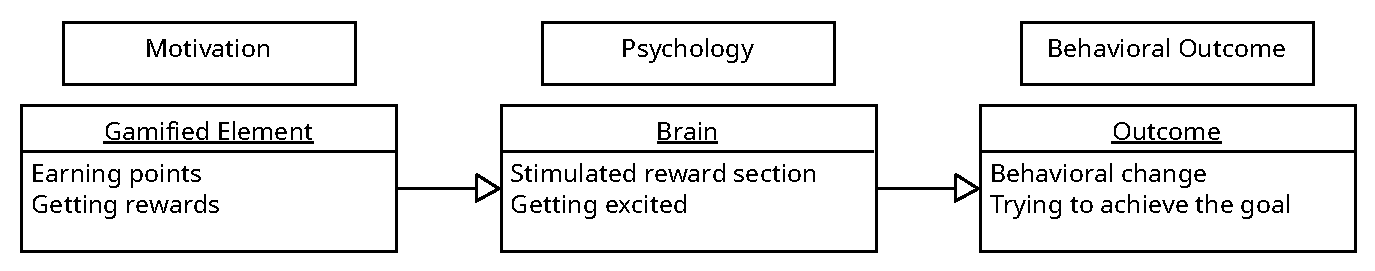
\includegraphics[width=1.0\linewidth]{Figure1.pdf}
\caption{How gamification works.}
\label{f:figure1}
\end{figure*}


Now, the meaning of gamification in health will be addressed \ref{G-i-H} and subsequently related benefits will be discussed in section ~\ref{benefits} . In section \ref{risks} risks and possible dangers connected to gamification will be examined. Finally, potential solutions for the challenges will be reviewed and final conclusions will be made  in summary. ~\ref{summary} .

%
%
%

\section{Gamification in health} \label{G-i-H}
Generally, the main goal of gamified elements in the context of health and well-being is changing user's behavior by increasing their activity and and/or practicing healthier life-style via game-like experience. The main reason why gamification is so popular in last years is strongly linked with the accessibility of digital technologies, particularly smart phones, as well as the created digital infrastructure\cite{Ethics} that has connected the world. 

The health trackers and health apps have millions of users today, and the competition in this field is enormous. In "Global Healthcare Gamification Market Analysis and Trends - Industry Forecast to 2025", research conducted by Research and Markets, the estimated market gap for gamification in healthcare is expected to reach \$13.58 billion by 2025 \cite{mgap} .  

Apple is one of the most significant examples of companies that implemented gamified elements successfully in their market strategies. The ecosystem created between user's Apple Watch and iPhone where user is rewarded for accomplishing tasks connected to movement - steps, calories and the count of hours user was active is one of the most used practice \cite{aboveAvalon} of gamification in terms of behavioral change and motivation.  Apple also rewards people on special days. For example, on the Earth Day (April 22.) the user can get a 'special' badge for exercising more than 30 minutes in that day\cite{earthDay}. 

%
%
%

\section{Benefits} \label{benefits}
The concept of implementing game-like elements in different areas of healthcare and well being has been talked about for some years and there are companies that managed to implement them successfully. This implementation opens up many ways to encourage users to be involved with their own health.  

\subsection{Healthier life-style } \label{lifestyle}
The use of technologies increased exponentially in last two decades. In general, IT sector has been linked with a more sedentary lifestyle of people of all generations. Therefore, many studies and researches tried to endorse the activity among users of technologies\cite{GONZALEZ2016529}. For example, companies like Nintendo (Wii) or Microsoft (Kinect) started to promote physical activity by including body movement as a gamified element in their apps.

Similarly, companies like Strava or Garmin are trying to get people moving. For example, in Strava, users have new challenges every month to keep them running, walking or cycling on a regular basis. Also Garmin encourages users to move and rewards them with virtual badges in their apps. Another successful app is Sweatcoin. This app rewards users with different discounts, coupons or even cash, purely for walking.

\subsection{Education of medical students} \label{stuff}
In the medical curriculum, games, mobile apps, and virtual patient simulations may be utilized to enhance learning, engagement, cooperation, real-world application, clinical decision making, distance training, learning analytics, and quick feedback\cite {https://doi.org/10.1002/ca.23916}.

Implementation of the elements mentioned above helps to make the education process affordable, students are more engaged and they can learn, for example, dangerous procedures, in simulated, safe  environment.

The table \ref{f:table 1} bellow shows the most common games and mobile apps, and advantages of each platform\cite{https://doi.org/10.1002/ca.23916}.

\begin{figure*}[tbh]
\centering
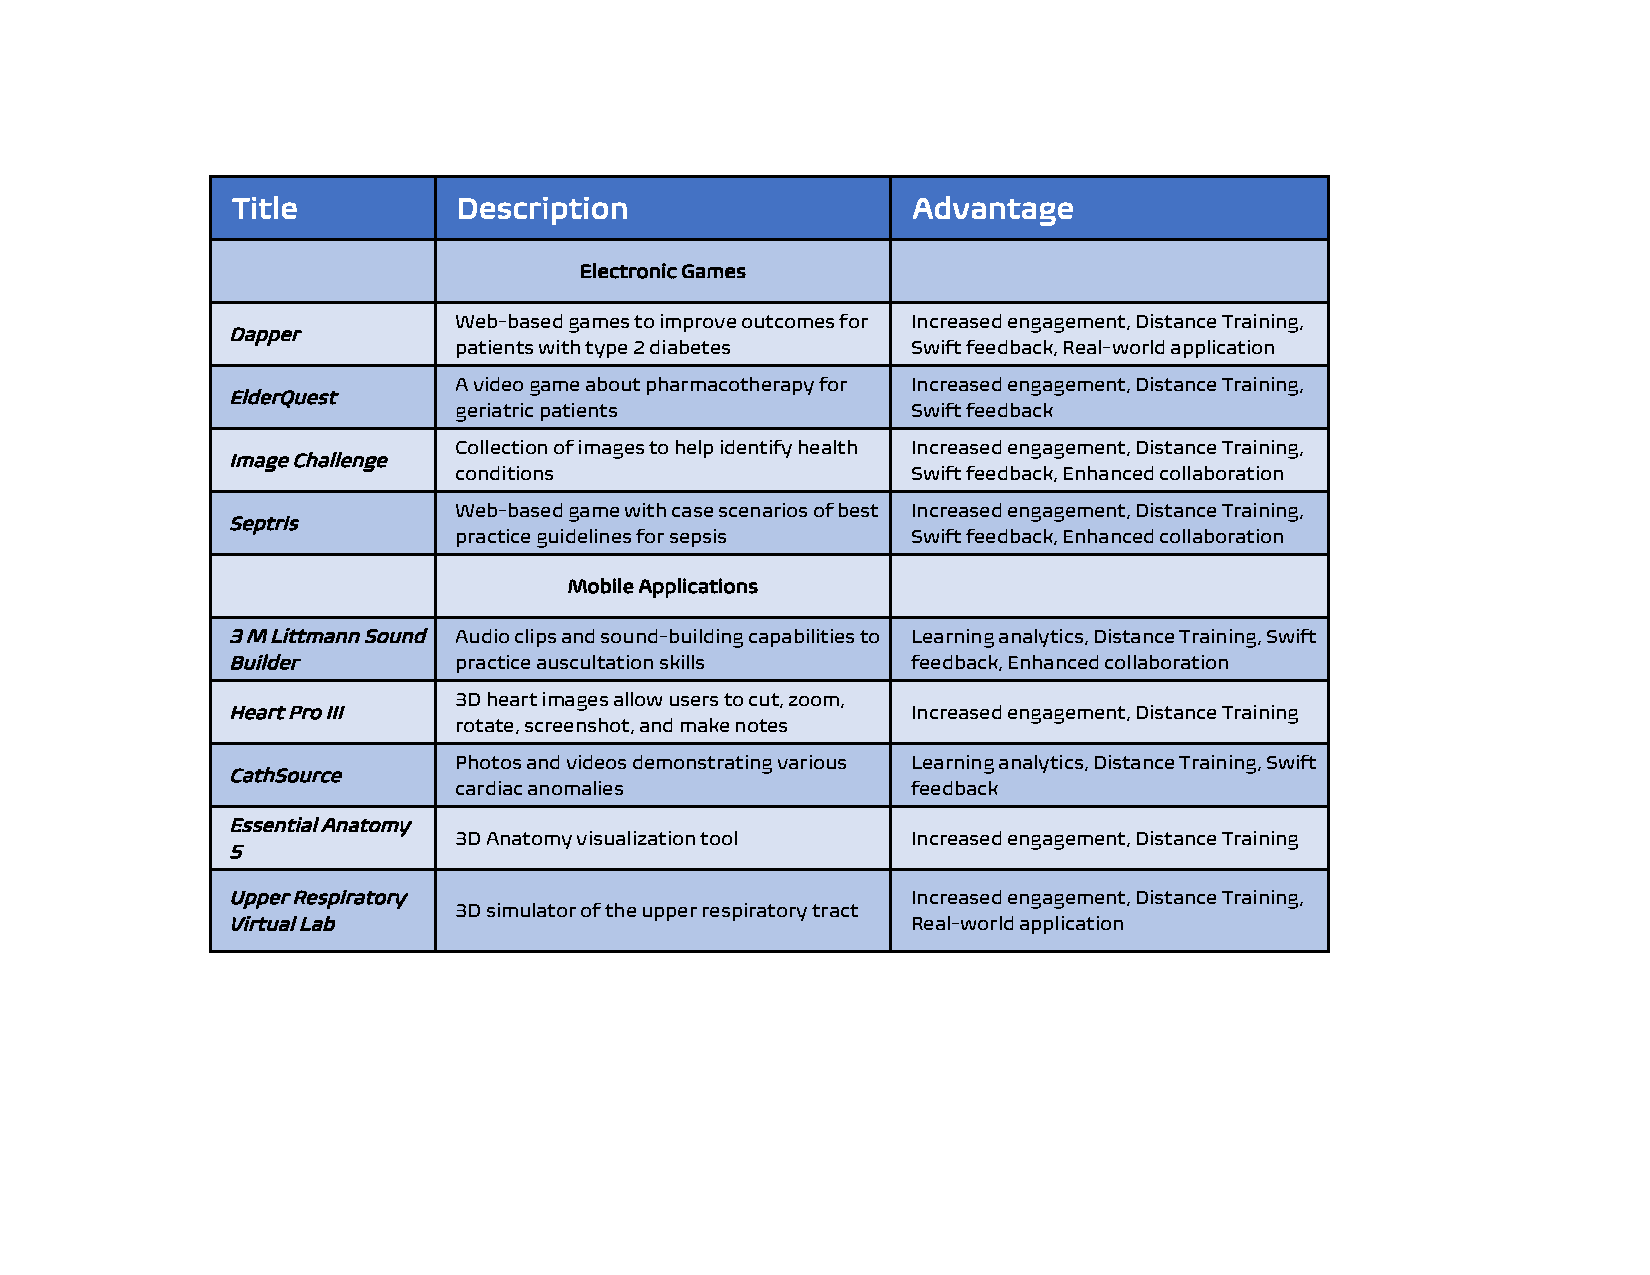
\includegraphics[width=1.0\linewidth]{table1.pdf}
\caption{The most used applications for education of medical students}
\label{f:table 1}
\end{figure*}



\subsection{Digitization of medical records} \label{bureau}
Nowadays, there are still many important documents that are stored in paper form. It can be medical records of patients, list of medical equipment in hospitals or prescriptions from a doctor. We can already notice that some of these are being replaced with online form - prescriptions. 

Digitization is helping to search through the documents faster, there is less probability of lost records or prescriptions. Also, if data are used correctly the human race can benefit from it in indirect ways. For example AI can learn to recognize some patterns of diseases which can be found in database of medical records of people suffering from these illnesses. Furthermore, digitization reduces usage of paper which means that less forests are cut down, which has a positive impact on global climate as well \cite{Digitization}.


%
%
%

\section{Risks and possible solutions} \label{risks}
As with everything, when humanity tries something new, there are some people who find ways to misuse it. That is the reason, why every computer has to use antivirus to be protected from malicious threads which hackers and scammers are using to damage your computer or steal your information.

This also applies on implementation of gamified elements in healthcare. There are many risks and potential problems which can occur. This article will discuss the  three most probable which the technology has to deal with.

\subsection{Privacy}\label{privacy}
The privacy problems created the crucial gap in the safety of digitization. Almost every application requires  the user to create a profile to interact with them. Thus, the user is asked to input information which can be in some cases misused. For example, applications can sell your e-mail address to third parties which will then use it for marketing. Also medical institutes are vulnerable to hackers or scammers practices.

To solve this problem the researches are proposing using of anonymity or pseudonymity to protect user's identity. Also, unlinkability is often used so the third parties cannot link any relationship between users or messages between them. Another method that helps is undetectability, which means that existence of a user or their information cannot be detected by a third party. \cite{fi11030067}. 

\subsection{Medical records} \label{records}
Similarly, the data about a patient as name, date of birth, identification number or other sensitive information, for example about parents or children are stored in databases. This data could be sold in some markets, thus, hackers often aim for such information \cite{fi11030067}. 

The best way to protect any information stored online is encrypting. Nowadays, there are many companies which offer great products for encrypting data also, the computer science courses teach encrypting and decoding in schools. The most important step in online safety is to stay updated. This means that the programmer should not just write an app or store data, but they should keep in mind how to protect them.

\subsection{Addiction} \label {addiction}
In the figure~\ref{f:figure1} above, we could see that receiving rewards is linked with dopamine production in the reward centre of one's brain; which can lead to addiction on such rewards, even without the designer intending that be the case.

A solution that Kim and Werbach proposed is to set some usage limits in the apps. This should not affect how difficult it is to achieve the goal, so users will not stop using the app because their goals are unreachable. Also, the programmer intention should be to motivate users' increased activity and not their time spent on the phone \cite{Kim2016}. 

%
%
%


\section{Summary} \label{summary} 
The aim of this paper was to analyse the benefits and risks connected with implementation of gamified elements in healthcare and overall health of the population. With the rise of technology and usage of mobile phones, it is important to motivate, not only young people, but every generation to move more, not forget to drink enough water and sleep appropriate among of time. Gamified health and fitness apps are designed to help user with everyday motivation. Gamification also helps to educate medical students in new ways, which can be cheaper and safer than real life application of the same procedure. Equally, digitization of medical records contributes to quicker processing and browsing data.

This article also proposed solutions to the most obvious problems which can be caused by gamification and digitization. The ethical issues with breaches in privacy and misuse of sensitive medical records can be solved by encryption of data. Likewise, the reward system may cause unintentional addictions. This can be easily solved by limitation of usage.

Overall, benefits of gamification outweigh the potential risks. However, in today's 'digital' world, it is important to implement them in the right manner and with ethics in programmer's mind. 

%
%
%

\section{Lecture topics}\label{prednasky}
\subsection{Sustainability and ethics}
It is very important to keep ethics in mind in today's world as the user became 'the goods' of the social platforms as well as web pages. The motivation of programmer should not just be the money, but also he should think how his product can affect users both in a good and bad way.
\subsection{History of computer science, people and technology}
The computer science as academic discipline started to appear in the 1950s. It came a long way in the form we know it today. The advance in computer science is exponential and people have to learn how to use new technologies. The technology is inseparable part of everyday life and the whole world is depending on it currently.



%\acknowledgement{Ak niekomu chcete poďakovať\ldots}


% týmto sa generuje zoznam literatúry z obsahu súboru literatura.bib podľa toho, na čo sa v článku odkazujete
\bibliography{lit1}
\bibliographystyle{plain} % prípadne alpha, abbrv alebo hociktorý iný
\end{document}
